\documentclass[11pt,letterpaper]{article}
\usepackage[utf8]{inputenc}
\usepackage{amsmath}
\usepackage{amsfonts}
\usepackage{amssymb}
\usepackage[margin=1in]{geometry}
\usepackage{graphicx}
\usepackage{placeins}
\usepackage{float}
\usepackage{listings}

\begin{document}
\noindent Landon Carter \\
9/29/16
6.111 PS5

\section{}
\subsection{A}
I took this image before realizing that I could just use a registered $\texttt{state}$, so the state numbers can actually just be 000, 001, 010, 011, and 100, respectively, rather than the one-hot encoding. This is reflected in the code.
\begin{figure}[H]
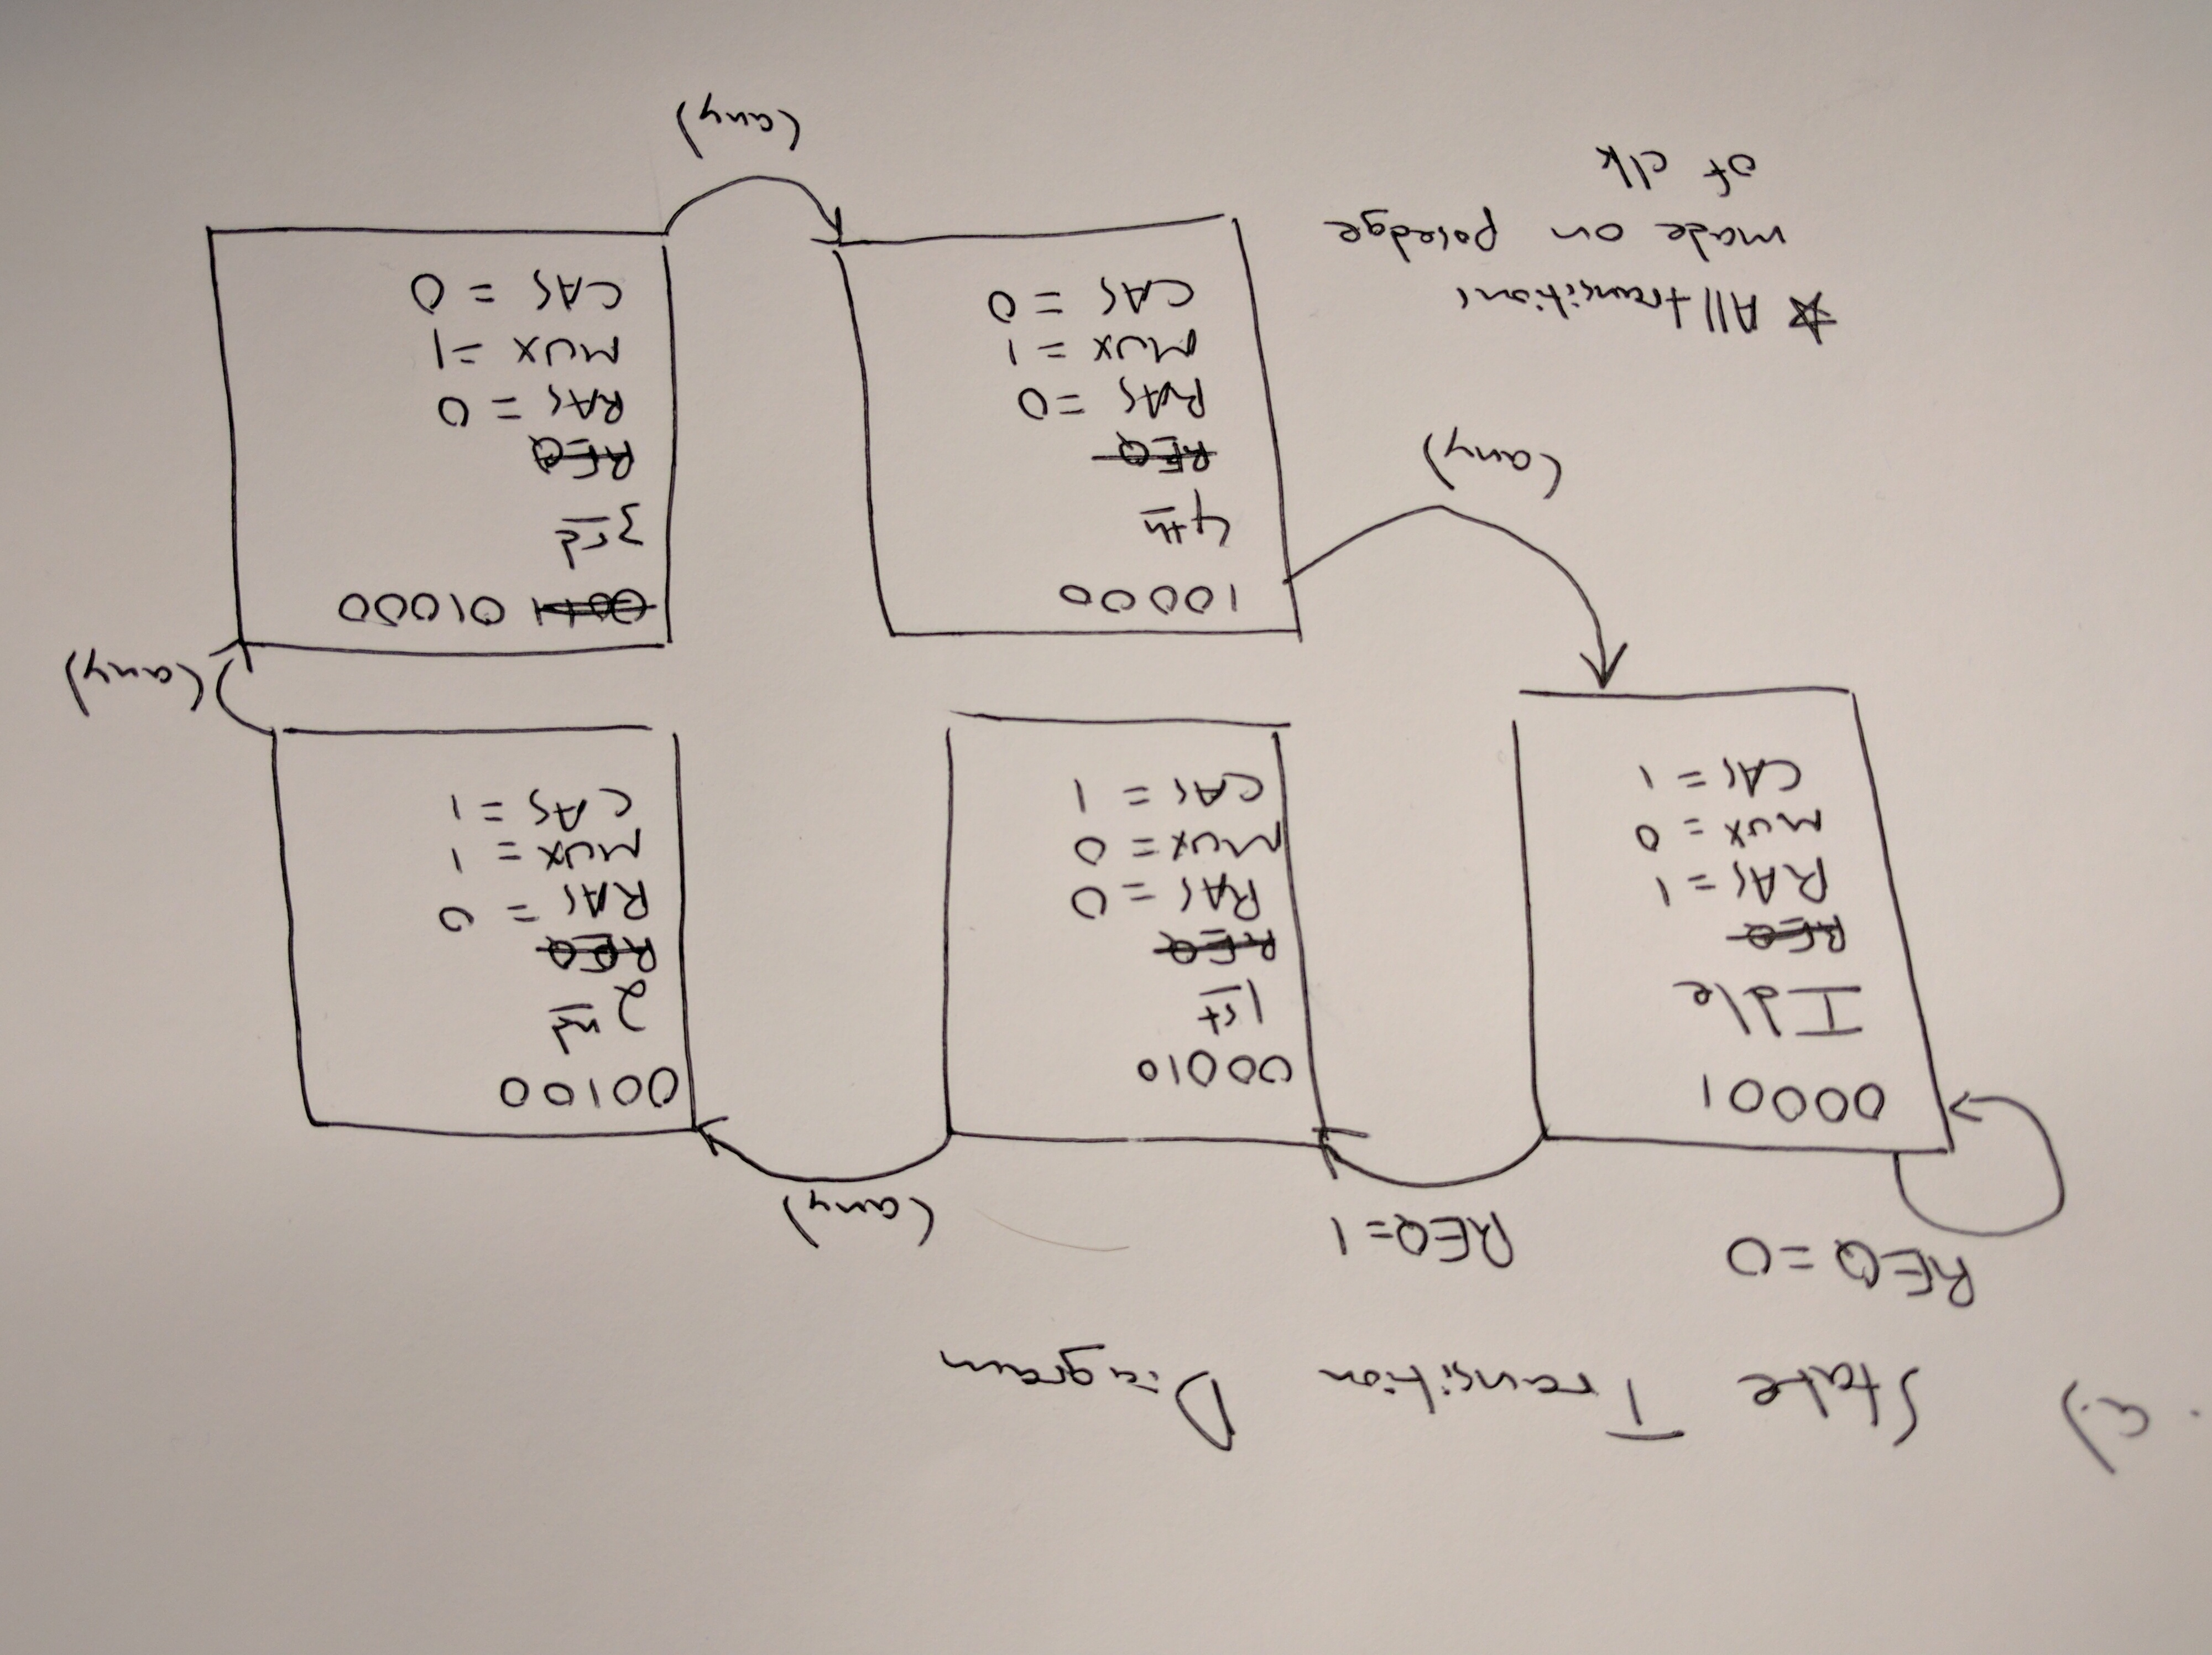
\includegraphics[width=6.5in]{state_transition.png}
\end{figure}

\subsection{B}
\begin{lstlisting}[language=Verilog]
module ps5(
    input req,
    input clk,
    output ras,
    output mux,
    output cas
    );
	 
	 parameter S_IDLE   = 0;
	 parameter S_1      = 1;
	 parameter S_2      = 2;
	 parameter S_3      = 3;
	 parameter S_4      = 4;

	reg [4:0] state, next_state;
	always @(*) begin
		case (state)
			S_IDLE: next_state = req ? S_1 : S_IDLE;
			S_1: next_state = S_2;
			S_2: next_state = S_3;
			S_3: next_state = S_4;
			S_4: next_state = S_IDLE;
			default: next_state = S_IDLE;
		endcase
	end
	always @(posedge clk) state <= next_state;
	
	assign ras = (state == S_IDLE);
	assign mux = !(state == S_IDLE || state == S_1);
	assign cas = !(state == S_3 || state == S_4);

endmodule

\end{lstlisting}

\section{C}
$\texttt{RAS}$, $\texttt{CAS}$, and $\texttt{MUX}$ are controlled by combinational logic dependent on $\texttt{state}$, which is a register assigned sequentially. Therefore, we don't need to worry about glitches, just a delay. In this implementation, $\texttt{next\_state}$ is set combinationally, so when $\texttt{state}$ is set sequentially on that, there is no delay - it's assigned on the next rising clock edge. (Additionally, and more practically, we can check the test output to confirm that is is not delayed).

\section{D}
\begin{lstlisting}[language=Verilog]
module ps5_tb;

	// Inputs
	reg req;
	reg clk;

	// Outputs
	wire ras;
	wire mux;
	wire cas;

	// Instantiate the Unit Under Test (UUT)
	ps5 uut (
		.req(req), 
		.clk(clk), 
		.ras(ras), 
		.mux(mux), 
		.cas(cas)
	);

	always #5 clk = !clk;  // 10 ns clk
	initial begin
		// Initialize Inputs
		req = 0;
		clk = 0;

		// Wait 100 ns for global reset to finish
		#100;
		
		#2; // Wait part of a clk cycle
		// Pulse req
		req = 1;
		#10;
		req = 0;

	end
      
endmodule
\end{lstlisting}
\begin{figure}[H]
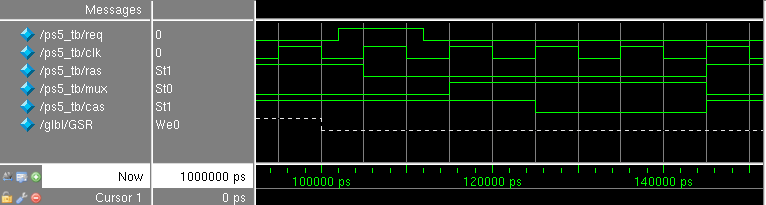
\includegraphics[width=6.5in]{wave.png}
\end{figure}



\end{document}
